\chapter{Process}
\label{chap:process}

\section{Scrum}
\label{sec:sysDevMethod}
This project used Scrum with 4 week sprints and resulted in a total of 3 sprints. Each sprint started after a meeting with the product owner. During these meetings, different tasks and challenges for the sprint were discussed in addition to their prioritization. After this meeting, the team had a meeting without the product owner where tasks were estimated. After the first sprint, the estimation tool Planningpoker \cite{Plann81:online} was used as other teams reported that they were very satisfied with this tool during the retrospective meetings. 

\section{Tools}
\label{sec:tools}

\begin{figure}[h]
  \centering
  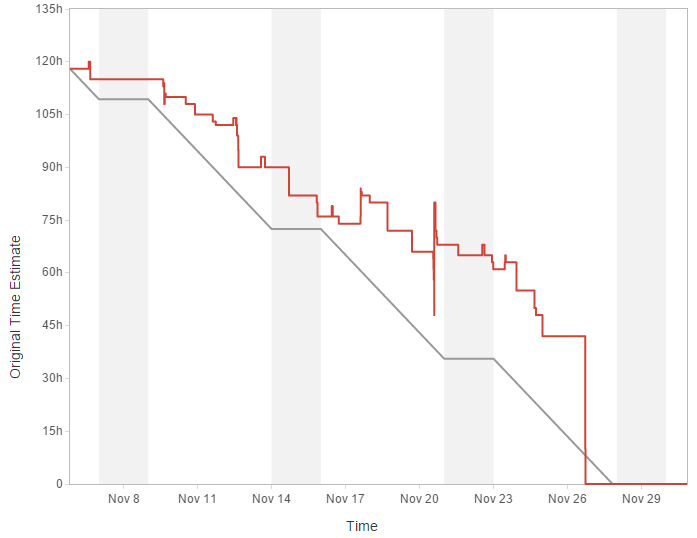
\includegraphics[width=.5\textwidth]{figures/sprint_burndown.png}
  \caption[Sprint burndown.]{Sprint burndown chart of the last sprint in this project.}
  \label{fig:sprintBurndown}
\end{figure}

JIRA was used as task management and time tracking of the project. This system managed all the tasks in the project such as their state, assignee, description, estimation, etc. It also managed the sprint and maintained a scrumboard in addition to a sprint burndown chart (See Figure \ref{fig:sprintBurndown}). Confluence was used more as a wiki where information such as project description, user stories and meeting notes were listed.

The team decided to set up an automated build server after the first sprints in order to make the project better comply with one of the learning outcomes of this course: "[...] knowledge in tools and methodologies used to develop “state-of-the-art” computer applications" \cite{Gjovi52:online}. Having an automated build server also made the development easier as it would automate the process of building and running tests and analysis on the code. Bamboo \cite{Bamboo} was used as the build server as another team were already using it and was recommending it due to the integration with JIRA and BitBucket (Cloud git service for the project repositories). Although integration was set up between these tools, some functionality between JIRA and BitBucket such as smart commits \cite{JiraSmartCommits} were limited as team members used different emails and/or usernames on the different services. However, integration worked well enough such that git commits could be tagged with a JIRA issue number so that an issue on JIRA would have a commits history. 

Skype was primarily used as the communication platform between the team members. Towards the end, the team started using Slack after a meeting with the supervisor where Slack was recommended. Comparing these two services, Slack becomes more team oriented as each team member does not maintain their own contact list but has a global list of all the users using Slack in their respective organization. It also maintains file transfers and conversation differently compared to Skype which has a synchronization approach which is not very reliable under certain circumstances.

For each commit that was made, the build server would be triggered from BitBucket. It would then build the project, run the unit tests in the project and run static code analysis using Sonar \cite{Sonar98:online}. If the build failed, the build server would display that the build was failed. A better integration with the Build server would be if it could notify the team members either through email or through Slack once the build failed. Therefore, the build server had to be checked manually. 

Sonar was also checked manually but more frequently towards the end of the project where more refactoring took place. The default rules for Java was applied once Sonar was introduced to the project, however more comprehensive rules from checkstyle \cite{checkStyle:online} was applied towards the end in order to better comply with Java conventions regarding formatting. Sonar was only used on the API, while JSHint was used on the Angular application. For further reference, see Section~\ref{sec:angularImpl}.